\documentclass[UTF8,12pt]{ctexart}

\usepackage[a4paper,margin=2.45cm]{geometry}
\usepackage{amsmath,amssymb}
\usepackage{booktabs,threeparttable,longtable,array,tabularx}
\usepackage{graphicx,float}
\usepackage{caption,subcaption}
\usepackage{setspace}
\usepackage{xcolor}
\usepackage{enumitem}
\usepackage{microtype}
\usepackage[colorlinks=true,linkcolor=black,citecolor=black,urlcolor=blue]{hyperref}
\usepackage[backend=biber,style=authoryear-comp,maxcitenames=2,maxbibnames=99,uniquelist=false]{biblatex}
\addbibresource{green_credit_transition_refs.bib}

\captionsetup{font=small,labelsep=quad}
\setlength{\tabcolsep}{4pt}
\renewcommand{\arraystretch}{1.13}
\onehalfspacing
\setlist{nosep,leftmargin=2em}
\setlength{\emergencystretch}{2em}

\newcommand{\sym}[1]{\rlap{#1}}
\newcommand{\note}[1]{\begin{minipage}{0.96\textwidth}\footnotesize\textit{注：}#1\end{minipage}}

\title{绿色信贷与高煤炭地区转型的边界：\\基于连续煤炭暴露度与地方路径的证据}
\author{王思涵\quad 刘伊然\quad 娄满榆\quad 赵佑恩}
\date{}

\begin{document}
\maketitle

\begin{abstract}
本文考察2012年《绿色信贷指引》实施后，政策前煤炭暴露度不同的省份在哪些调整边际上出现差异，以及这些差异是否延伸到能源资本和发电结构。本文使用中国省级年度面板，将政策后指标与2008--2011年煤炭终端消费占五类能源终端消费的平均比重相互作用，构造连续暴露度双重差分。基准结果显示，高煤炭暴露省份在政策后出现更明显的能源和煤炭终端强度下降，煤炭消费占比也下降；污染排放的基准关联在差异趋势控制下不稳定。全样本中加入煤炭暴露度与线性时间趋势的交互后，两项能源强度仍为负且显著，但完整的省份线性趋势会削弱这些估计，直接绿色信贷代理也未提供明确的金融渠道验证。因此，结果应理解为与绿色信贷约束一致的差异化政策后变化，而非排除同期政策的单一因果效应。二氧化碳排放、火电装机占比和火电发电占比没有出现稳定的同步差异。由政策前非火电装机与2013--2016年风电基础构成的“早期清洁电力基础”没有稳定放大后期新能源替代；三重交互项为负还可能包含基数效应和增长空间差异。晋蒙文本比较的稳定差异集中在绿色金融和煤炭清洁治理议题，而污染治理和新能源议题的省际差异不显著。总体而言，现有证据显示2012年后的省际响应在运行强度、能源使用构成与资本替代之间存在层级差异。绿色信贷更适合被理解为高煤炭地区转型的一项外部金融约束。

\noindent\textbf{关键词：}绿色信贷；煤炭暴露；能源强度；碳锁定；区域禀赋；政策文本
\end{abstract}

\section{引言}

绿色投资同时面临环境外部性、信息不对称和回收周期较长的问题。污染成本未被完全计入私人决策时，市场会系统性低估清洁投资的社会回报\parencite{pigou1920}；银行又可能因无法准确识别借款人的环境风险和转型质量而实施信贷配给\parencite{stiglitzweiss1981}。在以银行融资为主的经济体中，将环境与社会风险纳入授信标准，因而可能成为价格型环境政策之外的重要治理工具\parencite{campiglio2016,dikauvolz2021}。中国银监会于2012年发布《绿色信贷指引》，要求银行把环境与社会风险纳入贷前审查、授信审批和贷后管理，并对高耗能、高污染和产能过剩行业实施差异化信贷管理\parencite{cbrc2012}。

现有研究主要从企业融资、绿色创新、环境绩效和碳排放等角度评估这一政策。早期研究记录了中国绿色信贷制度从政策倡议向银行流程管理的转变\parencite{aizawayang2010,zhangyangbi2011}，后续研究则发现绿色信贷会改变受限行业的融资成本、债务期限和投资行为\parencite{cuietal2018,xuli2020}。近年来的准实验研究进一步报告了企业碳排放强度、污染治理、环境绩效和绿色创新等结果，但方向和作用渠道并不完全一致\parencite{xuyetal2023,wuetal2023,zhangetal2024green,laietal2024,lietal2024,pengetal2024,machen2025,zhengetal2025,zhangetal2025micro}。这类研究回答了绿色信贷是否影响企业，却较少区分高煤炭地区的不同调整层级。

这种区分具有实质意义。高煤炭地区可以在不立即退出煤炭和火电资本的情况下，通过降低能源投入强度、缩减高排放活动或安装治理设备来满足合规要求。煤炭消费占比也可能因天然气、电力或其他能源使用增加而下降，但这仍不必然意味着火电资本存量、发电结构和碳排放路径已经重组。大型能源资产具有不可逆性、长寿命和网络互补性，既有技术、基础设施和制度安排会共同产生锁定\parencite{arthur1989,david1985,unruh2000}。因此，绿色信贷首先改变运行边际，并不保证随后自动出现结构替代。

地方能源基础又使这种转换更复杂。传统资源经济学说明不可再生资源存量会塑造投资和开采路径\parencite{hotelling1931}，资源诅咒文献则指出资源依赖可能通过产业集中、财政依赖和制度激励限制新路径形成\parencite{auty1993,sachswarner2001}。另一方面，风光资源和早期清洁电力基础只是潜在机会。地区能否把外部政策信号转化为新产业和项目，还取决于知识相关性、吸收能力、基础设施和政策协调\parencite{cohenlevinthal1990,hidalgoetal2007,neffkeetal2011,boschma2017,hansencoenen2015}。这意味着“煤炭资源丰富”与“风光基础较好”都不能单独决定转型结果。

本文据此提出一个层级化研究问题：2012年后，政策前煤炭暴露度较高的省份首先在哪些边际上出现更明显变化？这些变化是否从运行强度和污染排放延伸到煤炭使用构成、碳排放和火电结构？早期清洁电力基础与资源依赖是否稳定改变这种延伸？本文使用2000--2023年省级面板，将2012年后指标与政策前煤炭终端消费占比相互作用，并结合连续暴露度事件研究、替代暴露度、差异趋势、绿色信贷水平代理、资源依赖指标和晋蒙政策文本进行分层检验。

本文的贡献有三点。第一，本文把结果变量区分为\textbf{运行性调整、构成性调整和结构替代}。这一分类不是按显著性事后排列，而是由调整成本和资产不可逆性推导：能源投入和排放可以通过行为调整较快变化，煤炭使用比例位于中间层，火电资本与新能源项目体系的调整最慢。第二，本文把绿色信贷和地方能源禀赋两条文献连接起来，检验外部金融约束是否在不同煤炭暴露和早期清洁电力基础下呈现不同层级，而不把“有风光基础”直接等同于完整的地方能力。第三，本文主动报告识别边界。补充事件研究显示核心能源强度存在政策前差异，省份趋势模型也明显削弱部分结果；可观测绿色信贷代理未验证一条清楚的政策渠道。因而本文的核心结论是分层事实与作用边界，不是绿色信贷单一政策的强因果效应。

\section{文献综述与理论框架}

\subsection{绿色信贷：从环境外部性到信贷配置}

环境经济学首先把污染理解为私人边际成本与社会边际成本之间的偏离\parencite{pigou1920}。传统政策主要通过税、排放标准或交易制度把外部成本内部化；绿色信贷进一步把环境风险纳入资本价格和可得性。信贷市场存在信息不对称时，银行不会只用利率清算市场，还会通过额度、期限和准入条件分配资金\parencite{stiglitzweiss1981}。一旦监管要求银行识别环境风险，污染记录和行业属性就可能改变贷款筛选、风险权重和贷后监督。这一机制说明绿色信贷既是融资工具，也是环境规制的金融执行形式\parencite{campiglio2016,dikauvolz2021}。

中国经验文献大体形成三组发现。第一组关注制度执行。\textcite{aizawayang2010}和\textcite{zhangyangbi2011}指出，绿色信贷的关键不只在优惠资金规模，还在于银行是否把环保信息嵌入授信流程。第二组关注融资后果。绿色贷款占比与银行风险之间存在差异\parencite{cuietal2018}，而《绿色信贷指引》对高污染企业的债务成本和期限产生非对称影响\parencite{xuli2020}。第三组关注企业真实行为。已有研究发现绿色信贷可能影响可再生能源投资、企业碳强度、创新和环境绩效\parencite{heetal2019,xuyetal2023,wuetal2023}。2024--2025年的研究进一步考察污染治理、环境绩效、绿色转型、金融韧性和企业碳强度，显示政策效果会随所有制、融资约束、监管环境和企业能力而异\parencite{zhangetal2024green,laietal2024,lietal2024,pengetal2024,machen2025,zhengetal2025,zhangetal2025micro}。

这组研究提供了绿色信贷能够影响微观融资与环境行为的证据，但不能直接推出省级能源结构会同步变化。企业可以通过缩减产量、改变能源投入、购买成熟治理设备或重新分类项目来应对授信约束；这些反应的成本和时间均低于建设新能源项目、并网和退出火电资产。因此，企业层面的“有效”与地区能源结构的替代并不是同一个命题。

\subsection{调整成本、诱致创新与结构替代}

环境规制是否提升生产率，长期存在“合规成本”与“创新补偿”两种机制。波特假说认为设计合理的规制可能诱导创新并部分抵消合规成本\parencite{portervanderlinde1995}，但研发投入和专利反应并不必然立即转化为生产率\parencite{jaffepalmer1997}。诱致创新和定向技术变迁模型进一步表明，相对价格和政策会改变技术搜索方向，但既有知识存量会使技术响应具有路径依赖\parencite{popp2002,acemogluetal2012,aghionetal2016}。可再生能源政策对专利的影响也随技术类型和政策工具而变化\parencite{johnstoneetal2010}。

这些理论共同推出一个调整顺序。本文将\textbf{运行性调整}定义为在既有煤炭体系内部改变投入和排放边际，包括五类能源终端强度、煤炭终端强度和污染排放；将\textbf{构成性调整}定义为煤炭在能源使用中的比例变化；将\textbf{结构替代}定义为火电资本、发电结构、碳排放路径与新能源项目体系的持续重组。运行性调整不要求资本退出，构成性调整可能由多种能源共同变化产生，结构替代则需要新资本形成、网络接入与旧资本退出。由此得到第一个理论预期：金融约束更可能首先出现在运行边际，结构变量的变化更慢、也更依赖其他政策与地方条件。

\subsection{地方能源禀赋、锁定与区域能力}

不可再生资源会影响地区的产业、财政和就业结构\parencite{hotelling1931,auty1993,sachswarner2001}。当煤炭开采、火电、运输和地方财政形成互补关系后，技术收益递增与协调成本会强化既有路径\parencite{arthur1989,david1985,unruh2000}。可持续转型研究因此强调，技术替代是技术、市场、基础设施和制度共同演化的过程\parencite{geels2002,markardetal2012}，且不同地区的知识基础、产业相关性和政策能力会产生不同路径\parencite{hansencoenen2015,boschma2017}。

吸收能力理论指出，利用外部知识取决于既有知识和组织能力\parencite{cohenlevinthal1990}；产品空间和区域相关性研究也表明，地区更容易进入与既有能力相近的新活动\parencite{hidalgoetal2007,neffkeetal2011}。绿色技术同样具有这种相关性，政治支持只能在既有知识和产业条件上发挥作用\parencite{santoalhaboschma2021}。近期研究进一步发现，资源依赖对可再生能源发展的作用可能是非线性的，并随政策支持变化\parencite{zhangetal2024resource}；“棕色”地区进入绿色技术的路径取决于其经济实力和知识组合\parencite{grashofbasilico2025}；煤炭地区的转型还必须处理就业、财政和区域公平\parencite{healybarry2017,carleyetal2018,demeterova2024,tassikittner2024,perettoetal2025}。最新的区域吸收能力研究也把政策效果理解为外部政策与本地技术基础的共同产物\parencite{zhaoetal2026}。

这些研究同时否定两种简单决定论。煤炭资源丰富不必然使绿色政策失效，因为资源收入、产业技术和基础设施也可能被重新利用；风光资源或早期风电基础较好也不必然产生更快增长，因为高基数、消纳约束和项目周期会限制边际扩张。本文因此把政策前非火电装机和2013--2016年风电基础称为“早期清洁电力基础”，而不称为自然禀赋或完整地方能力。

\subsection{研究缺口与可检验预期}

绿色信贷文献主要检验企业融资和环境结果，区域转型文献主要讨论资源依赖、技术相关性和地方能力。两者之间仍有三个缺口。第一，全国性金融规制在煤炭暴露不同的地区究竟先影响哪一类结果，缺少统一的层级比较。第二，煤炭占比下降是否与碳排放、火电资本和发电结构同步，常被“绿色转型”这一总括概念遮蔽。第三，既有清洁电力基础是否足以把金融约束转化为新能源替代，缺少与高煤炭暴露同时考虑的检验。

本文提出三个有方向但有边界的经验预期：其一，2012年后，高煤炭暴露省份可能先出现运行强度和部分污染排放的差异化下降；其二，煤炭占比可能出现构成性调整，但结构替代变量未必同步；其三，早期清洁电力基础只是潜在前置条件，其与煤炭暴露的三重交互方向并不预先设定，因为先发优势与高基数、消纳约束可以同时存在。本文以这些预期组织证据，而不把任何单一不显著系数解释为“没有影响”。

\section{制度背景、数据与研究设计}

\subsection{制度背景与识别对象}

《绿色信贷指引》于2012年2月发布，要求银行识别、计量、监测和控制信贷活动中的环境与社会风险，并根据风险性质和严重程度调整授信审批、合同和贷后管理\parencite{cbrc2012}。政策在全国同时生效，因而不存在天然的未受政策省份。本文使用政策前煤炭暴露度刻画潜在处理强度：煤炭在终端能源使用中占比越高，地方工业和能源活动与受限行业的联系通常越紧密，政策后融资和合规环境的变化也可能更具约束性。

这一设计识别的是2012年后不同政策前煤炭暴露省份的\textbf{差异化变化}，并不直接观测银行收紧了多少绿色信贷。2012年后还存在节能目标、煤炭消费控制、大气污染防治、供给侧改革和地方产业政策，它们可能同样对煤炭省份产生差异影响。省份和年份固定效应不能排除这些并行政策。为此，本文把连续双重差分称为主政策后比较，并用事件研究、差异趋势、替代暴露度和可观测绿色信贷代理评估其可信度，而不把政策名称本身当作渠道已经得到验证。

\subsection{样本与数据来源}

基础面板覆盖中国内地31个省级地区的2000--2023年，共744个省份--年份观测。由于环保财政支出和市场化指数等控制变量自2007年后覆盖较完整，主回归的实际窗口通常为2007--2023年；五类能源变量止于2022年。各表报告实际样本量和估计年份。

宏观变量来自《中国统计年鉴》及Wind整理的国家统计局省级序列。能源变量来自《中国能源统计年鉴》地区能源平衡表及其Wind导出序列。五类能源包括煤炭、油品、液化石油气、天然气和电力；它们不是全部一次能源，因此本文始终称为“五类能源口径”。原始物理量按统一折标准煤系数汇总：煤炭、油品、液化石油气、天然气和电力分别依据原始单位转换为万吨标准煤。电力装机和发电量来自《中国电力统计年鉴》及Wind分地区序列；环境排放来自《中国环境统计年鉴》和生态环境统计资料。二氧化碳序列为基于EDGAR 2024（v8.0）网格数据汇总的省级化石能源与工业过程排放，单位为吨\parencite{crippaetal2024}。

绿色信贷补充指标来自用户提供的《2005--2022年绿色信贷水平》工作簿，覆盖31省。原表的实际口径为六大高耗能行业利息费用占规模以上工业企业利息费用的比重，本文构造正向代理：
\begin{equation}
\begin{aligned}
\text{绿色信贷代理}_{it}
  =1-\frac{\text{六大高耗能行业利息费用}_{it}}
  {\text{规模以上工业企业利息费用}_{it}}.
\end{aligned}
\end{equation}
该变量越高，表示高耗能行业在工业利息费用中的份额越低。它反映工业融资结构，不是监管口径的省级绿色贷款余额；2017年由源工作簿插值，因而补充结果同时剔除2017年。

晋蒙政策文本来自山西省和内蒙古自治区政府网站公开文件。清洗后山西有3,874份文件，内蒙古有2,974份文件，覆盖2000--2023年。本文将标题、主题和正文合并，对绿色金融、煤炭清洁治理、污染治理和新能源四组词典计数，并构造每万字词频与至少提及一次该主题的政策文件比例。关键词计数不识别语义方向，两个网站的历史归档口径也不完全一致，因此文本只刻画政策注意力，不表示政策支持强度。

\subsection{变量构造与概念对应}

政策前煤炭暴露度定义为2008--2011年煤炭终端消费占五类能源终端消费的平均比重：
\begin{equation}
\begin{aligned}
\text{煤炭暴露}_{i}
  =\frac{1}{4}\sum_{s=2008}^{2011}
  \frac{\text{煤炭终端消费}_{is}}
  {\text{五类能源终端消费}_{is}}.
\end{aligned}
\end{equation}
样本中该指标的省级均值为0.415，标准差为0.149，范围为0.102--0.644。主解释变量为“2012年后×煤炭暴露”。煤炭暴露不随时间变化，其水平项被省份固定效应吸收。

运行性调整包括五类能源终端消费/GDP、煤炭终端消费/GDP，以及工业二氧化硫、氮氧化物和工业固废排放。由于现有项目未保存省级GDP平减指数，强度指标使用名义GDP；本文补充使用能源量取对数并控制GDP的模型，检验分母口径是否驱动结果。原面板中的绿色全要素生产率和全局曼奎斯特--卢恩伯格指数因缺少可完整复现的投入、期望产出和非期望产出源文件，只在附录报告，不承担主结论。

构成性调整包括五类能源口径煤炭占比和原统计口径煤炭消费占比。结构替代包括二氧化碳排放对数、火电装机占比、火电发电占比、非火电发电占比、风电发电占比、风光发电占比和风电装机占比。表\ref{tab:mapping}说明概念与证据等级。

\begin{table}[H]
\centering
\caption{调整层级与变量对应}
\label{tab:mapping}
\begin{tabularx}{\textwidth}{p{2.7cm}p{4.5cm}X p{2.5cm}}
\toprule
层级 & 理论含义 & 对应变量 & 证据定位 \\
\midrule
运行性调整：强度 & 既有能源体系内部降低投入强度 & 五类能源终端强度、煤炭终端强度 & 基准证据；动态和趋势敏感 \\
运行性调整：排放 & 排放活动、产量或治理设备共同变化 & 工业SO$_2$、NO$_x$、工业固废，附带颗粒物和废水 & 基准关联；趋势下不稳定 \\
构成性调整 & 煤炭在能源使用中的相对比重变化 & 五类能源煤炭占比、原煤炭消费占比 & 动态较规整；趋势下不稳定 \\
结构替代：深层 & 火电资本、发电结构和碳路径同步重组 & CO$_2$、火电装机占比、火电发电占比 & 边界证据；火电发电有前趋势 \\
结构替代：新能源 & 新能源装机、发电和项目体系扩张 & 非火电、风电、风光发电占比和风电装机占比 & 探索性条件证据 \\
地方路径 & 地方政策议程与后验能源表现 & 晋蒙文本词频、覆盖比例和阶段均值 & 描述性案例证据 \\
\bottomrule
\end{tabularx}
\end{table}

“早期清洁电力基础”由三个指标标准化后取均值：2008--2011年非火电装机占比、2013--2016年风电装机占比和2013--2016年风电发电占比。其公式为：
\begin{equation}
\begin{aligned}
\text{早期清洁电力基础}_{i}
=\frac{1}{3}\big[&z(\text{政策前非火电装机}_{i})
+z(\text{早期风电装机}_{i})\\
&+z(\text{早期风电发电}_{i})\big].
\end{aligned}
\end{equation}
后两个成分发生在2012年之后，因而该指数不是严格外生的政策前禀赋，只能描述2016年前已经形成的清洁电力基础。资源依赖指数则由政策前采矿就业占比、煤炭采选业资产占比和资源税依赖标准化后取均值，并以加入煤炭产量依赖的四维版本作替代定义。

\subsection{模型设定}

主模型为省份和年份双向固定效应：
\begin{equation}
\begin{aligned}
Y_{it}={}&\beta(\text{政策后}_{t}\times\text{煤炭暴露}_{i})
+\gamma'X_{it}+\mu_i+\lambda_t+\varepsilon_{it},
\end{aligned}
\label{eq:did}
\end{equation}
其中，$X_{it}$包括地区生产总值对数、人口、第二产业占比、城镇化率、环保财政支出占比和市场化指数；$\mu_i$和$\lambda_t$分别为省份和年份固定效应。标准误聚类到省份层面。$\beta$表示高一单位政策前煤炭暴露对应的政策后差异，而不是绿色信贷余额增加一单位的效应。

事件研究将2011年作为基准期，并把2008年及以前、2016年及以后分别合并：
\begin{equation}
\begin{aligned}
Y_{it}={}&\sum_{\tau\neq -1}\beta_{\tau}
\left(\text{煤炭暴露}_{i}\times\mathbf{1}[t-2012=\tau]\right)\\
&+\gamma'X_{it}+\mu_i+\lambda_t+\varepsilon_{it}.
\end{aligned}
\label{eq:event}
\end{equation}
政策前系数的联合检验用于评估差异趋势。鉴于主回归实际从2007年开始，最早一档只有有限年份，事件研究的检验力和解释均需保持克制。

新能源结果使用2016年后指标，完整保留可识别的低阶交互项：
\begin{equation}
\begin{aligned}
Y_{it}={}&\beta_1(\text{2016年后}_{t}\times\text{煤炭暴露}_{i})\\
&+\beta_2(\text{2016年后}_{t}\times\text{早期清洁基础}_{i})\\
&+\theta(\text{2016年后}_{t}\times\text{煤炭暴露}_{i}
\times\text{早期清洁基础}_{i})\\
&+\gamma'X_{it}+\mu_i+\lambda_t+\varepsilon_{it}.
\end{aligned}
\label{eq:ddd}
\end{equation}
“煤炭暴露×早期清洁基础”不随时间变化，被省份固定效应吸收。$\theta$只说明高煤炭暴露与早期清洁基础的组合是否对应不同的2016年后变化，不能单独识别资源、项目或电网渠道。

晋蒙文本模型为$\text{内蒙古}\times\text{2012年后}$的两省固定效应比较。样本只有两个省，且网站归档口径不同，因此不作因果解释。

\section{实证结果}

\subsection{描述性统计}

表\ref{tab:desc}报告主要变量。煤炭暴露的省年均值为0.415，标准差为0.147。五类能源终端强度和煤炭终端强度的变异较大；风电和风光结果自2011年后覆盖较完整，因此有效样本明显少于其他变量。绿色信贷代理覆盖2005--2022年，共558个省年。

\begin{table}[H]
\centering
\caption{主要变量描述性统计}
\label{tab:desc}
\begin{tabular}{lrrrrr}
\toprule
变量 & 观测数 & 均值 & 标准差 & 最小值 & 最大值 \\
\midrule
政策前煤炭暴露 & 720 & 0.415 & 0.147 & 0.102 & 0.644 \\
五类能源终端强度 & 686 & 0.650 & 0.428 & 0.088 & 4.726 \\
煤炭终端强度 & 686 & 0.285 & 0.287 & 0.001 & 3.221 \\
工业SO$_2$ & 720 & 45.203 & 39.481 & 0.059 & 171.500 \\
NO$_x$ & 348 & 53.057 & 39.522 & 3.490 & 180.110 \\
工业固废 & 720 & 40.002 & 33.608 & 0.158 & 160.500 \\
五类能源煤炭占比 & 686 & 0.379 & 0.167 & 0.007 & 0.746 \\
CO$_2$排放对数 & 744 & 19.077 & 0.915 & 16.081 & 20.887 \\
火电装机占比 & 683 & 0.652 & 0.241 & 0.024 & 1.000 \\
火电发电占比 & 735 & 0.716 & 0.255 & 0.001 & 1.000 \\
风光发电占比 & 342 & 0.075 & 0.076 & 0.000 & 0.447 \\
绿色信贷代理 & 558 & 0.460 & 0.147 & 0.094 & 0.972 \\
\bottomrule
\end{tabular}
\end{table}

\subsection{运行性调整：能源强度与污染排放}

表\ref{tab:intensity}复现原基准结果。政策后煤炭暴露对五类能源终端强度的系数为$-0.2895$，在5\%水平显著；对煤炭终端强度的系数为$-0.4262$，在1\%水平显著。以煤炭暴露的一个省级标准差0.149计算，两项对应变化约为$-0.043$和$-0.064$个样本单位。绿色全要素生产率和全局ML指数均不显著，因而基准结果不能被表述为广义生产率提高。

\begin{table}[H]
\centering
\caption{政策后煤炭暴露与能源强度}
\label{tab:intensity}
\resizebox{0.96\textwidth}{!}{%
\begin{tabular}{lcccc}
\toprule
 & 绿色全要素生产率 & 全局ML指数 & 五类能源终端强度 & 煤炭终端强度 \\
\midrule
政策后煤炭暴露 & -1.0498 & -0.1342 & -0.2895** & -0.4262*** \\
 & (0.7528) & (0.0830) & (0.1190) & (0.0776) \\
样本量 & 510 & 510 & 480 & 480 \\
$R^2$ & 0.7644 & 0.2719 & 0.9592 & 0.9237 \\
省份/年份固定效应 & 是 & 是 & 是 & 是 \\
\bottomrule
\end{tabular}}
\note{括号内为省份聚类稳健标准误。***、**、*分别表示1\%、5\%、10\%显著性。前两列为不可完整复算的继承指标，仅作补充。}
\end{table}

污染排放结果见表\ref{tab:pollution}。工业SO$_2$、NO$_x$和工业固废的系数分别为$-72.5887$、$-43.9915$和$-47.2683$，均达到常规显著水平；颗粒物和工业废水不显著。这里的因变量是排放量，下降可能来自产出收缩、产业转移、燃料替代或末端治理，因而表题和解释使用“污染排放响应”，不把系数直接等同于治理投资增加。

\begin{table}[H]
\centering
\caption{政策后煤炭暴露与污染排放响应}
\label{tab:pollution}
\resizebox{\textwidth}{!}{%
\begin{tabular}{lccccc}
\toprule
 & 工业SO$_2$ & NO$_x$ & 颗粒物 & 工业固废 & 工业废水 \\
\midrule
政策后煤炭暴露 & -72.5887*** & -43.9915** & -10.1339 & -47.2683** & -40594.6149 \\
 & (19.6996) & (16.8916) & (28.0627) & (20.0521) & (24203.0698) \\
样本量 & 510 & 336 & 154 & 510 & 510 \\
$R^2$ & 0.8812 & 0.9223 & 0.8225 & 0.7837 & 0.9108 \\
省份/年份固定效应 & 是 & 是 & 是 & 是 & 是 \\
\bottomrule
\end{tabular}}
\note{括号内为省份聚类稳健标准误。污染排放下降不能单独识别末端治理渠道。}
\end{table}

\subsection{构成性调整与结构替代边界}

表\ref{tab:structure}把煤炭使用构成和深层结构变量并列。五类能源煤炭占比和原煤炭消费占比的系数分别为$-0.2495$和$-0.1900$，均在1\%水平显著。CO$_2$排放、火电装机占比和火电发电占比的系数则均不显著。煤炭占比下降因此是构成性调整的证据，但不能被直接解释为火电体系退出。不显著结果同样不能证明政策“没有影响”：CO$_2$系数的95\%置信区间约为$[-0.310,0.113]$，火电装机和火电发电的区间也较宽，现有样本无法排除具有经济意义的正负变化。

机组级分析进一步检验煤炭暴露与资本退出之间是否存在稳定关联。基于GEM 2026年快照回溯的煤电机组投产与退役记录，本文将每台机组拆分为政策阶段内的风险区间，采用省份聚类稳健的左截断Cox比例风险模型，并控制机组容量和投产年份。以煤炭暴露的一个省级标准差为单位，政策前（2000--2011年）退役风险比为1.26（$p=0.063$）；2012--2015年为1.01（$p=0.955$），后续两个阶段也未达到常规显著水平。按样本中位数划分高、低煤组的辅助规格同样未得到稳定差异。该分析没有观察到2012年后高煤地区煤电退出加速的证据；由于阶段系数差异的聚类稳健检验力有限，它提供的是结构替代未获得直接支持的边界证据，而非绿色信贷改变煤电退出风险的因果识别。这一边界与省级面板中能源强度调整更早出现的模式相互呼应。

\begin{table}[H]
\centering
\caption{煤炭使用构成、碳排放与火电结构}
\label{tab:structure}
\begin{tabular}{lccccc}
\toprule
 & 五类能源 & 原口径 & CO$_2$ & 火电装机 & 火电发电 \\
 & 煤炭占比 & 煤炭占比 & 排放对数 & 占比 & 占比 \\
\midrule
政策后煤炭暴露 & -0.2495*** & -0.1900*** & -0.0982 & 0.0517 & 0.0888 \\
 & (0.0754) & (0.0651) & (0.1034) & (0.0945) & (0.0754) \\
样本量 & 480 & 480 & 510 & 510 & 507 \\
$R^2$ & 0.9224 & 0.9382 & 0.9904 & 0.9368 & 0.9478 \\
省份/年份固定效应 & 是 & 是 & 是 & 是 & 是 \\
\bottomrule
\end{tabular}
\note{括号内为省份聚类稳健标准误。}
\end{table}

\subsection{动态检验与稳健性：证据等级的重新划分}

补充诊断见表\ref{tab:diagnostics}和附录图\ref{fig:event}. 五类能源终端强度的政策前联合检验$p=0.052$，接近常规边界；煤炭终端强度$p=0.041$，拒绝政策前系数共同为零。全样本加入煤炭暴露度与线性年份趋势的交互后，五类能源强度和煤炭终端强度的系数分别为$-0.1133$（$p=0.025$）和$-0.0845$（$p=0.041$）。该设定控制的是暴露度相关的共同线性漂移；吸收完整的省份线性趋势后，前者仅在10\%水平边际显著，后者不再显著。两组趋势规格共同表明，强度变化更符合逐步展开的调整，不能据此消除省份差异趋势担忧。工业SO$_2$的政策前检验同样接近边界，省份趋势模型的系数转为显著正值。煤炭占比的事件研究较为规整：政策前联合检验$p=0.840$，政策后系数逐步转负，2016年以后合并项为$-0.3685$；但两种趋势规格下，其平均政策后系数均不显著。

\begin{table}[H]
\centering
\caption{事件研究与差异趋势诊断}
\label{tab:diagnostics}
\resizebox{\textwidth}{!}{%
\begin{tabular}{lrrrrr}
\toprule
结果变量 & 基准系数 & 政策前联合$p$ & 暴露度$\times$年趋势 & 省份趋势系数 & 剔除五个煤炭省系数 \\
\midrule
五类能源终端强度 & -0.2895** & 0.052 & -0.1133** & -0.1225* & -0.2622** \\
煤炭终端强度 & -0.4262*** & 0.041 & -0.0845** & -0.0574 & -0.3903*** \\
工业SO$_2$ & -72.5887*** & 0.053 & 15.6304 & 28.6158*** & -68.6357*** \\
五类能源煤炭占比 & -0.2495*** & 0.840 & 0.0509 & 0.0897 & -0.2191*** \\
CO$_2$排放对数 & -0.0982 & -- & -- & -0.0213 & 0.0044 \\
火电装机占比 & 0.0517 & -- & -- & 0.0808 & 0.0352 \\
火电发电占比 & 0.0888 & 0.002 & -- & -0.0943* & 0.0650 \\
\bottomrule
\end{tabular}
}
\note{暴露度$\times$年趋势列在双向固定效应基础上加入煤炭暴露度与线性年份趋势的交互；省份趋势列吸收各省线性趋势。剔除省份为山西、内蒙古、陕西、新疆和宁夏。火电发电占比存在明显政策前差异。}
\end{table}

名义GDP分母也可能影响强度指标。将五类能源终端量和煤炭终端量取对数、并在右侧控制GDP后，基准系数分别为$-0.6134$（$p<0.001$）和$-0.8496$（$p=0.056$）。然而，前者的事件研究政策前联合$p=0.014$，后者加入省份趋势后不显著；两项省份趋势系数均不显著。因此，替代口径没有消除差异趋势担忧。

替代暴露度也显示结果依赖于煤炭暴露的定义。用政策前火电发电占比、原煤产量全国份额或近期煤电投产占比替代煤炭终端占比时，两项能源强度和煤炭占比大多不显著；工业SO$_2$对政策前原煤产量份额仍为显著负值。综合而言，基准表展示了一组清楚的分层相关模式，但严格因果解释主要受政策前差异趋势和处理强度构造限制。后文据此使用“2012年后的差异化变化”，不再使用“绿色信贷导致”。

\subsection{早期清洁电力基础与新能源结果}

表\ref{tab:cleanbase}报告三重交互。2016年后×早期清洁电力基础对风光发电占比为$0.0908$，在10\%水平显著，说明早期基础较高省份后期风光占比总体增长较快。但三重交互在风电和风光发电占比上分别为$-0.0927$和$-0.2363$，均在5\%水平显著。这一结果只能说明：在煤炭暴露较高的省份，早期清洁电力基础没有对应更大的2016年后边际增幅。它可能反映高基数、剩余增长空间较小、弃风限电或项目时序，不能解释为清洁能源基础“阻碍”转型。

\begin{table}[H]
\centering
\caption{早期清洁电力基础与2016年后新能源变化}
\label{tab:cleanbase}
\begin{tabular}{lcccc}
\toprule
 & 非火电发电 & 风电发电 & 风光发电 & 风电装机 \\
 & 占比 & 占比 & 占比 & 占比 \\
\midrule
2016年后×煤炭暴露 & -0.2231* & 0.0024 & -0.0919 & 0.0273 \\
 & (0.1164) & (0.0240) & (0.0724) & (0.0675) \\
2016年后×早期清洁基础 & 0.1072 & 0.0309 & 0.0908* & 0.0246 \\
 & (0.0695) & (0.0182) & (0.0461) & (0.0329) \\
三重交互 & -0.1757 & -0.0927** & -0.2363** & -0.1077 \\
 & (0.1514) & (0.0402) & (0.1093) & (0.0821) \\
样本量 & 507 & 330 & 330 & 288 \\
$R^2$ & 0.9514 & 0.8916 & 0.8921 & 0.9311 \\
\bottomrule
\end{tabular}
\note{三重交互为“2016年后×煤炭暴露×早期清洁电力基础”。模型包含所有可识别低阶交互；不随时间变化的两两交互被省份固定效应吸收。}
\end{table}

现有电网数据不足以把负向交互归因于消纳。输出电量仅从2015年开始，风光利用小时从2018年开始，弃风弃光率从2020年开始。使用2015年“1--11月输出电量/全年发电量”近似早期外送条件时，外送条件的三重交互对风电装机、风电发电和风光发电占比均不显著。因此，电网、项目和外送只保留为理论上可能的解释，本文没有对其进行机制确认。

\subsection{资源依赖与绿色信贷代理：两个补充诊断}

资源依赖三重差分没有支持“资源依赖统一削弱政策效果”。表\ref{tab:resource}显示，资源依赖三重交互对能源强度、煤炭强度、煤炭占比和火电结构大多不显著；对NO$_x$为显著负值，对后期风光发电占比仅在10\%附近为负。加入煤炭产量依赖的四维指标后，能源和结构结果仍大多不显著。这更接近“资源依赖改变调整边际”，而不是单向资源诅咒。

\begin{table}[H]
\centering
\caption{资源依赖的探索性三重交互}
\label{tab:resource}
\resizebox{0.96\textwidth}{!}{%
\begin{tabular}{lrrr}
\toprule
结果变量 & 煤炭暴露项 & 资源依赖项 & 三重交互 \\
\midrule
五类能源终端强度 & -0.2996** & 0.0180 & -0.0690 \\
煤炭终端强度 & -0.4641*** & 0.0327 & -0.0738 \\
工业SO$_2$ & -85.1875*** & 14.3355 & -28.6690* \\
NO$_x$ & -54.3413*** & 14.6222* & -38.8085** \\
五类能源煤炭占比 & -0.3321*** & 0.0646 & -0.0676 \\
CO$_2$排放对数 & -0.2813 & 0.2805 & -0.4174 \\
火电装机占比 & 0.0941 & -0.0120 & -0.0349 \\
火电发电占比 & 0.1188 & 0.0078 & -0.0312 \\
2016年后风光发电占比 & -0.0955 & 0.0862** & -0.1437* \\
\bottomrule
\end{tabular}}
\note{资源依赖为政策前采矿就业、煤炭采选业资产和资源税依赖的标准化均值。该表是异质性探索，不识别资源依赖的外生变化。}
\end{table}

绿色信贷代理提供更直接但仍是相关性的金融端诊断。政策后煤炭暴露对绿色信贷代理的系数为0.0809（$p=0.401$），剔除2017年后为0.0810（$p=0.382$），均不显著。绿色信贷代理本身与能源强度、煤炭强度、工业SO$_2$和风光发电占比也没有稳定显著的当期或滞后关系；它与火电装机和火电发电占比反而呈显著正相关。由于代理由行业利息费用构造，可能同时受到企业利润、利率和产业周期影响，这些结果不能作结构解释。其主要作用是提醒：全国政策×煤炭暴露的主系数尚未得到可观测绿色信贷水平的清楚渠道验证。

\subsection{晋蒙政策文本：地方议题差异而非机制识别}

表\ref{tab:text}比较2012年后内蒙古相对山西的文本变化。稳定显著的差异集中在绿色金融和煤炭清洁治理：每万字词频分别提高0.3062和9.3511，政策覆盖比例分别提高0.0382和0.1361。污染治理和新能源词频及覆盖比例均不显著。阶段均值中，内蒙古后期新能源词频和风光发电占比确有上升，但两省固定效应回归没有识别出稳定的新能源议题差异。因此，文本证据只能说明地方政策议程不同，不能证明内蒙古已经形成由绿色信贷驱动的新能源替代路径。

\begin{table}[H]
\centering
\caption{晋蒙政策文本注意力差异}
\label{tab:text}
\begin{tabular}{lcccc}
\toprule
 & 绿色金融 & 煤炭清洁治理 & 污染治理 & 新能源 \\
\midrule
\multicolumn{5}{l}{\textit{A. 每万字词频}}\\
内蒙古×2012年后 & 0.3062* & 9.3511*** & 0.1263 & 1.2466 \\
 & (0.1577) & (2.4313) & (0.7338) & (1.6355) \\
\midrule
\multicolumn{5}{l}{\textit{B. 政策文件覆盖比例}}\\
内蒙古×2012年后 & 0.0382** & 0.1361*** & 0.0299 & 0.0102 \\
 & (0.0145) & (0.0398) & (0.0203) & (0.0167) \\
\midrule
样本量 & 44 & 44 & 44 & 44 \\
省份/年份固定效应 & 是 & 是 & 是 & 是 \\
\bottomrule
\end{tabular}
\note{样本仅包括山西和内蒙古。文本归档与文件类型可能存在省际差异；结果只解释为政策注意力。}
\end{table}

\section{讨论}

\subsection{能够支持的结论：2012年后响应具有层级差异}

各组结果共同呈现一个层级模式。基准模型中，能源投入强度、煤炭终端强度和部分污染排放首先下降；煤炭占比随后表现出最清楚的政策后动态；CO$_2$、火电装机和火电发电没有稳定同步变化；风光结果又受较晚的数据起点和高基数影响。这个顺序与调整成本理论一致：改变设备运行、能源投入和排放活动通常快于建设新电源、接入电网和退出长寿命火电资本\parencite{portervanderlinde1995,unruh2000,geels2002}。

但“与理论一致”不等于渠道已经得到识别。能源强度和工业SO$_2$存在政策前差异或趋势敏感性，替代暴露度也不能普遍复现结果。最准确的概括是：2012年后的省际差异集中在运行和煤炭使用构成，结构变量的证据更弱。本文不能据此把所有变化归因于《绿色信贷指引》，也不能把污染排放下降命名为末端治理投资增加。

\subsection{地方能源基础为何不是充分条件}

早期清洁电力基础的三重交互为负，并不支持“基础越好，绿色信贷越能促进新能源替代”的线性命题。它至少有三种相容解释。第一，早期风电占比高的省份剩余增长空间更小，负系数可能是收敛和基数效应。第二，装机和发电是资源、项目审批、并网和消纳共同作用的结果，2013--2016年的指标已经包含政策后选择。第三，煤炭暴露与风光基础并存的省份可能同时承担能源保供和跨省送电功能，新增可再生能源未必立即降低本地火电占比。

区域相关性和吸收能力理论说明，资源机会只有与知识、企业、基础设施和治理协调结合时才会转化为新路径\parencite{cohenlevinthal1990,boschma2017,santoalhaboschma2021,zhaoetal2026}。本文的数据只能测量早期清洁电力基础，不能测量完整的“地方承接能力”。现有输出电量、利用小时和弃风弃光率起点过晚，早期外送代理的三重交互又不显著。因此，项目建设、并网、外送和政策连续性应被视为下一步需要检验的条件，而不是本文已经证明的机制。

\subsection{晋蒙案例的有限功能}

山西和内蒙古都具有较高煤炭依赖，但案例证据的稳定部分不是“山西治理污染、内蒙古发展新能源”的二分法。2012年后，内蒙古相对山西更频繁出现绿色金融和煤炭清洁治理表述；污染治理和新能源文本差异不显著。内蒙古后期风光发电占比更高是一项描述性结果，不能与文本回归拼接为因果链。

两省仍具有解释价值，因为它们提醒全国平均模型之外存在地方议程和基础设施差异。山西的政策文本长期保留煤炭安全、先进产能和清洁利用议题，内蒙古后期同时出现更多风光基地和外送相关表述。这些差异适合用于提出机制假说，而不是验证机制。领导更替、环保督察和能源保供节点也只能作为历史背景；在没有外生政治变化和完整项目数据时，不进入主识别。

\subsection{与资源依赖命题的关系}

资源诅咒理论容易引出“资源依赖必然削弱绿色金融”的强预测，但本文结果不支持这一单向命题。资源依赖三重交互对多数结果不显著，对NO$_x$等污染指标反而更负，对风光发电则为边际负值。可观测绿色信贷代理与资源依赖的交互在部分强度结果上也呈负相关，而不是全面失效。这说明资源依赖可能改变政策作用落在哪个边际，却不能被压缩成一个统一的抑制系数。近期关于资源依赖与可再生能源非线性关系的研究同样强调政策支持和发展阶段\parencite{zhangetal2024resource}。

\section{结论与政策含义}

本文考察2012年后不同政策前煤炭暴露省份的分层变化。基准结果显示，高煤炭暴露省份的能源和煤炭终端强度下降更明显，煤炭消费占比也显著下降；CO$_2$排放、火电装机和火电发电占比没有稳定同步差异。能源强度在暴露度相关的共同线性趋势控制下仍为负，但完整的省份趋势会明显削弱估计；煤炭占比和污染结果也存在趋势敏感性。机组级退出分析未观察到2012年后高煤地区煤电退出加速。早期清洁电力基础没有稳定放大后期风光替代，资源依赖也没有表现出统一的负向调节。晋蒙文本的稳定差异集中在绿色金融和煤炭清洁治理，而不是新能源议题。

因此，本文最终支持的是\textbf{调整层级不同}，不是《绿色信贷指引》的无条件强因果效应。绿色信贷及同期绿色规制可以提高高煤炭活动的融资和合规约束，但运行强度变化、煤炭使用构成变化与能源资本替代是三个不同命题。煤炭占比下降是向结构替代靠近的信号，却不是结构替代完成的证据；早期风光基础提供机会，却不是后期增长的充分条件。

政策上，绿色金融应与地区所处的调整阶段匹配。对存量煤炭资产较重的地区，信贷约束需要与能效改造、污染控制、煤电灵活性改造、落后产能退出和劳动者再配置结合；对具有风光项目基础的地区，融资支持还需与并网、储能、外送和电力市场改革协同。只按项目是否已经“纯绿”筛选，可能既无法处理存量高碳资产，也无法为退出和替代提供连续融资。转型金融的作用在于把限制、改造、替代和退出纳入同一时间路径，而不是放松环境约束。

本文有四项明确限制。第一，全国政策与连续煤炭暴露的设计无法排除同期面向煤炭省份的其他政策；关键结果的政策前趋势并不全部满足。第二，能源强度使用名义GDP，替代的能源量模型也未消除趋势担忧。第三，绿色信贷代理是高耗能行业利息费用的反向指标，现有工具变量第一阶段较弱，不能用于因果识别。第四，项目、电网、外送和消纳数据起点较晚，政策文本又不能识别语义方向。未来研究需要银行--企业贷款匹配、政策前电网能力、项目级建设时点和更长的新能源数据，才能检验金融约束如何真正转化为结构替代。

\appendix
\section{连续暴露度事件研究图}

\begin{figure}[H]
\centering
\begin{subfigure}{0.49\textwidth}
\centering
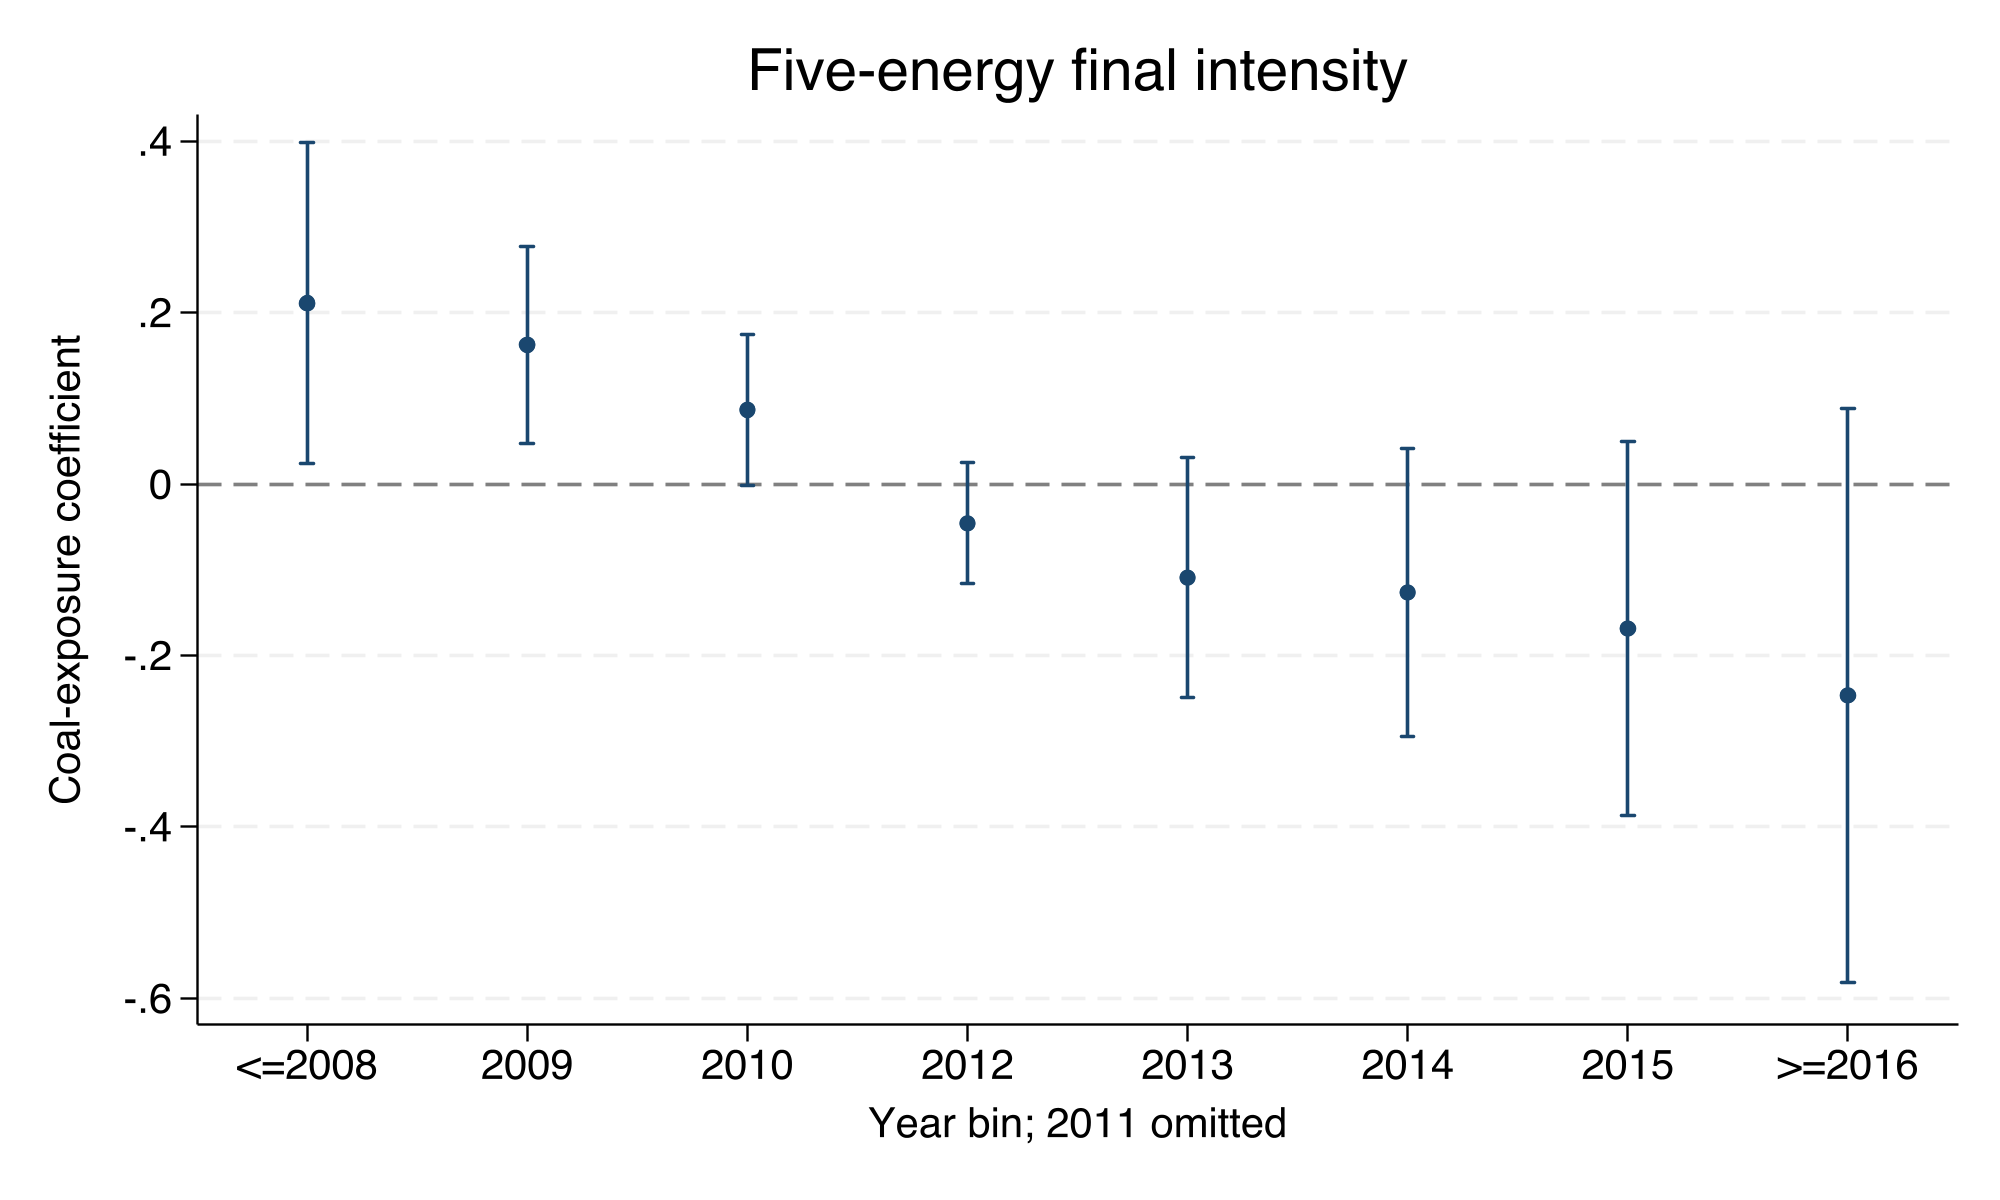
\includegraphics[width=\linewidth]{../result/figures/0718_manuscript_revision/EventStudy_energy5_int.png}
\caption{五类能源终端强度}
\end{subfigure}
\begin{subfigure}{0.49\textwidth}
\centering
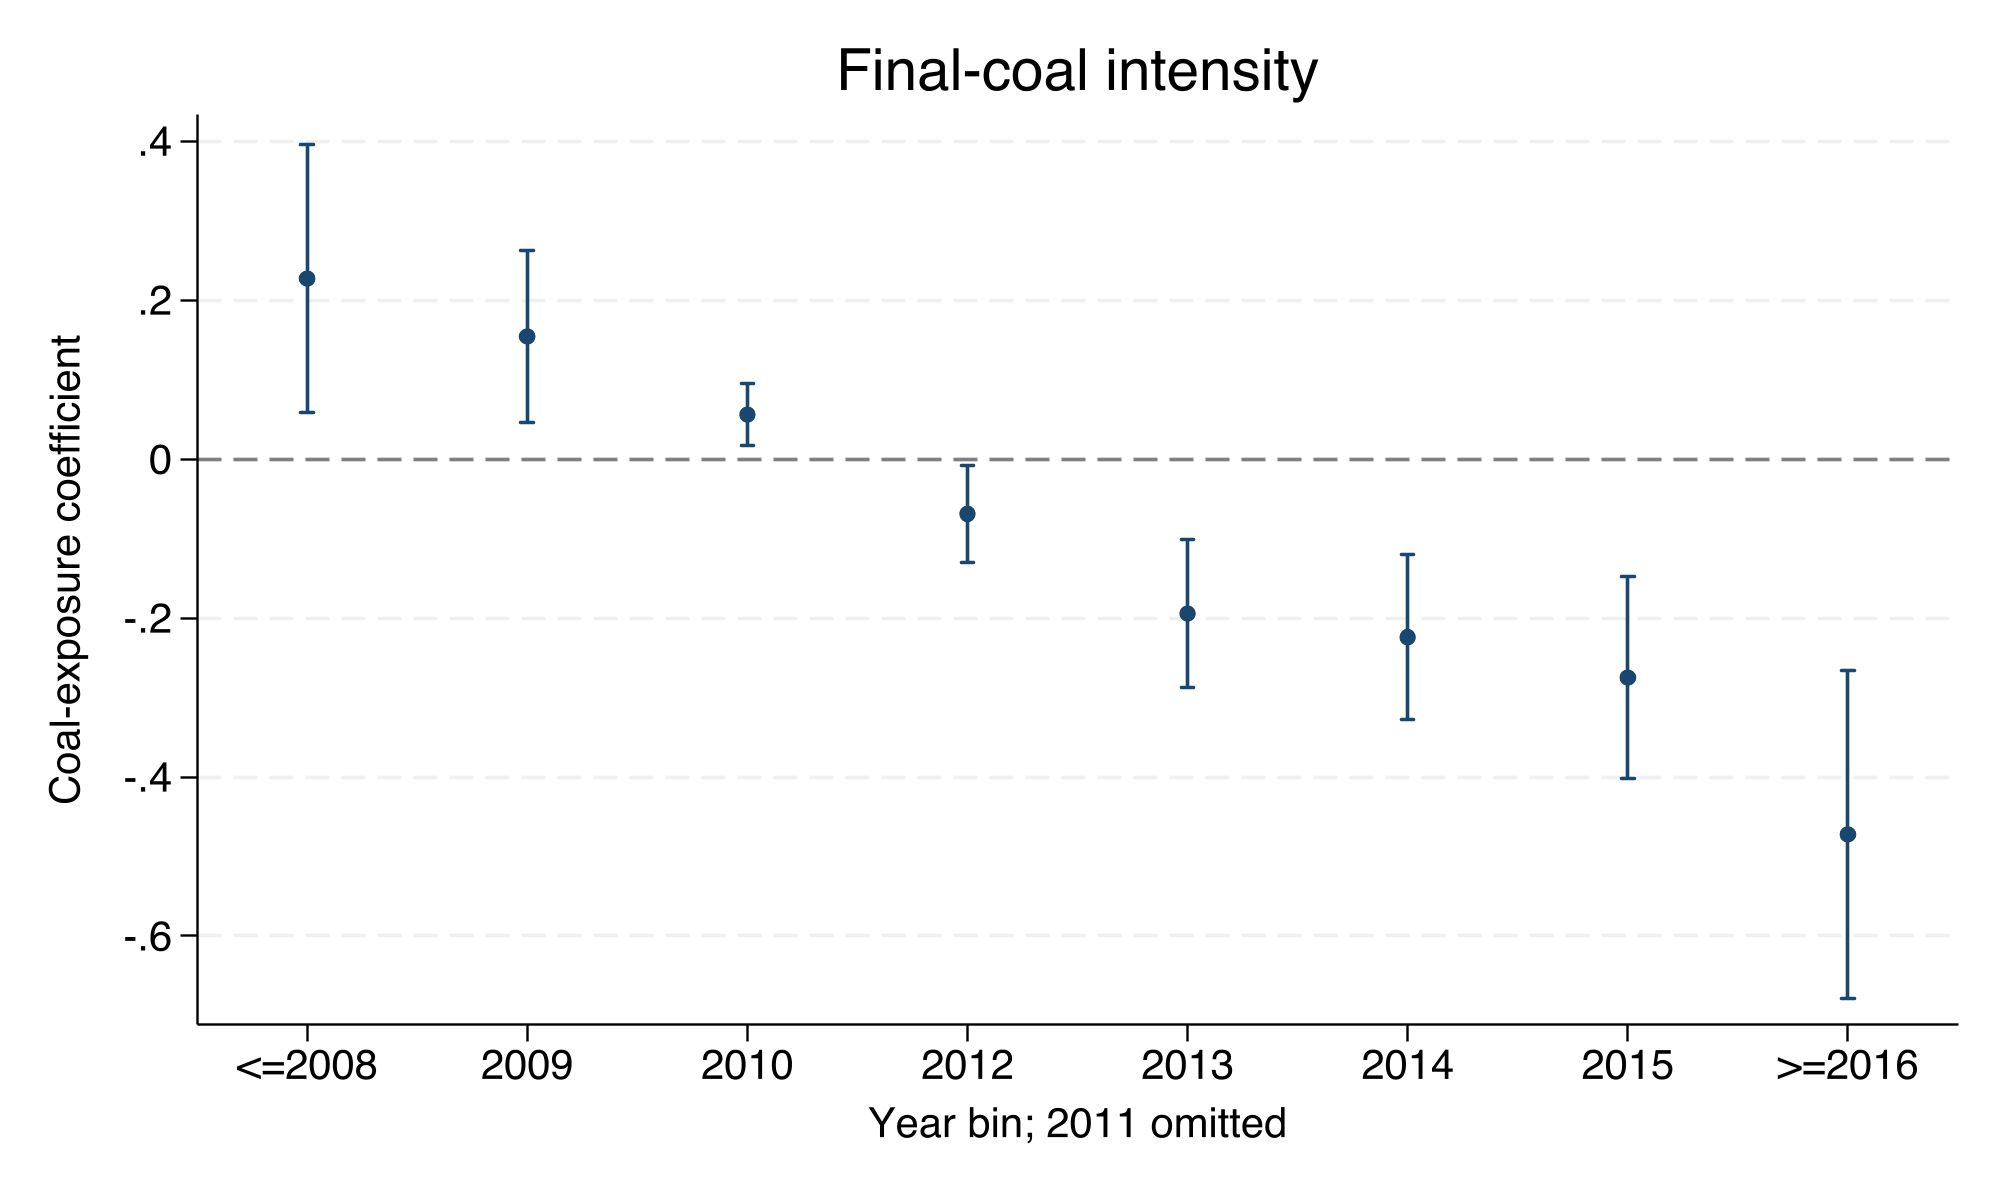
\includegraphics[width=\linewidth]{../result/figures/0718_manuscript_revision/EventStudy_coalterm_int.png}
\caption{煤炭终端强度}
\end{subfigure}

\begin{subfigure}{0.49\textwidth}
\centering
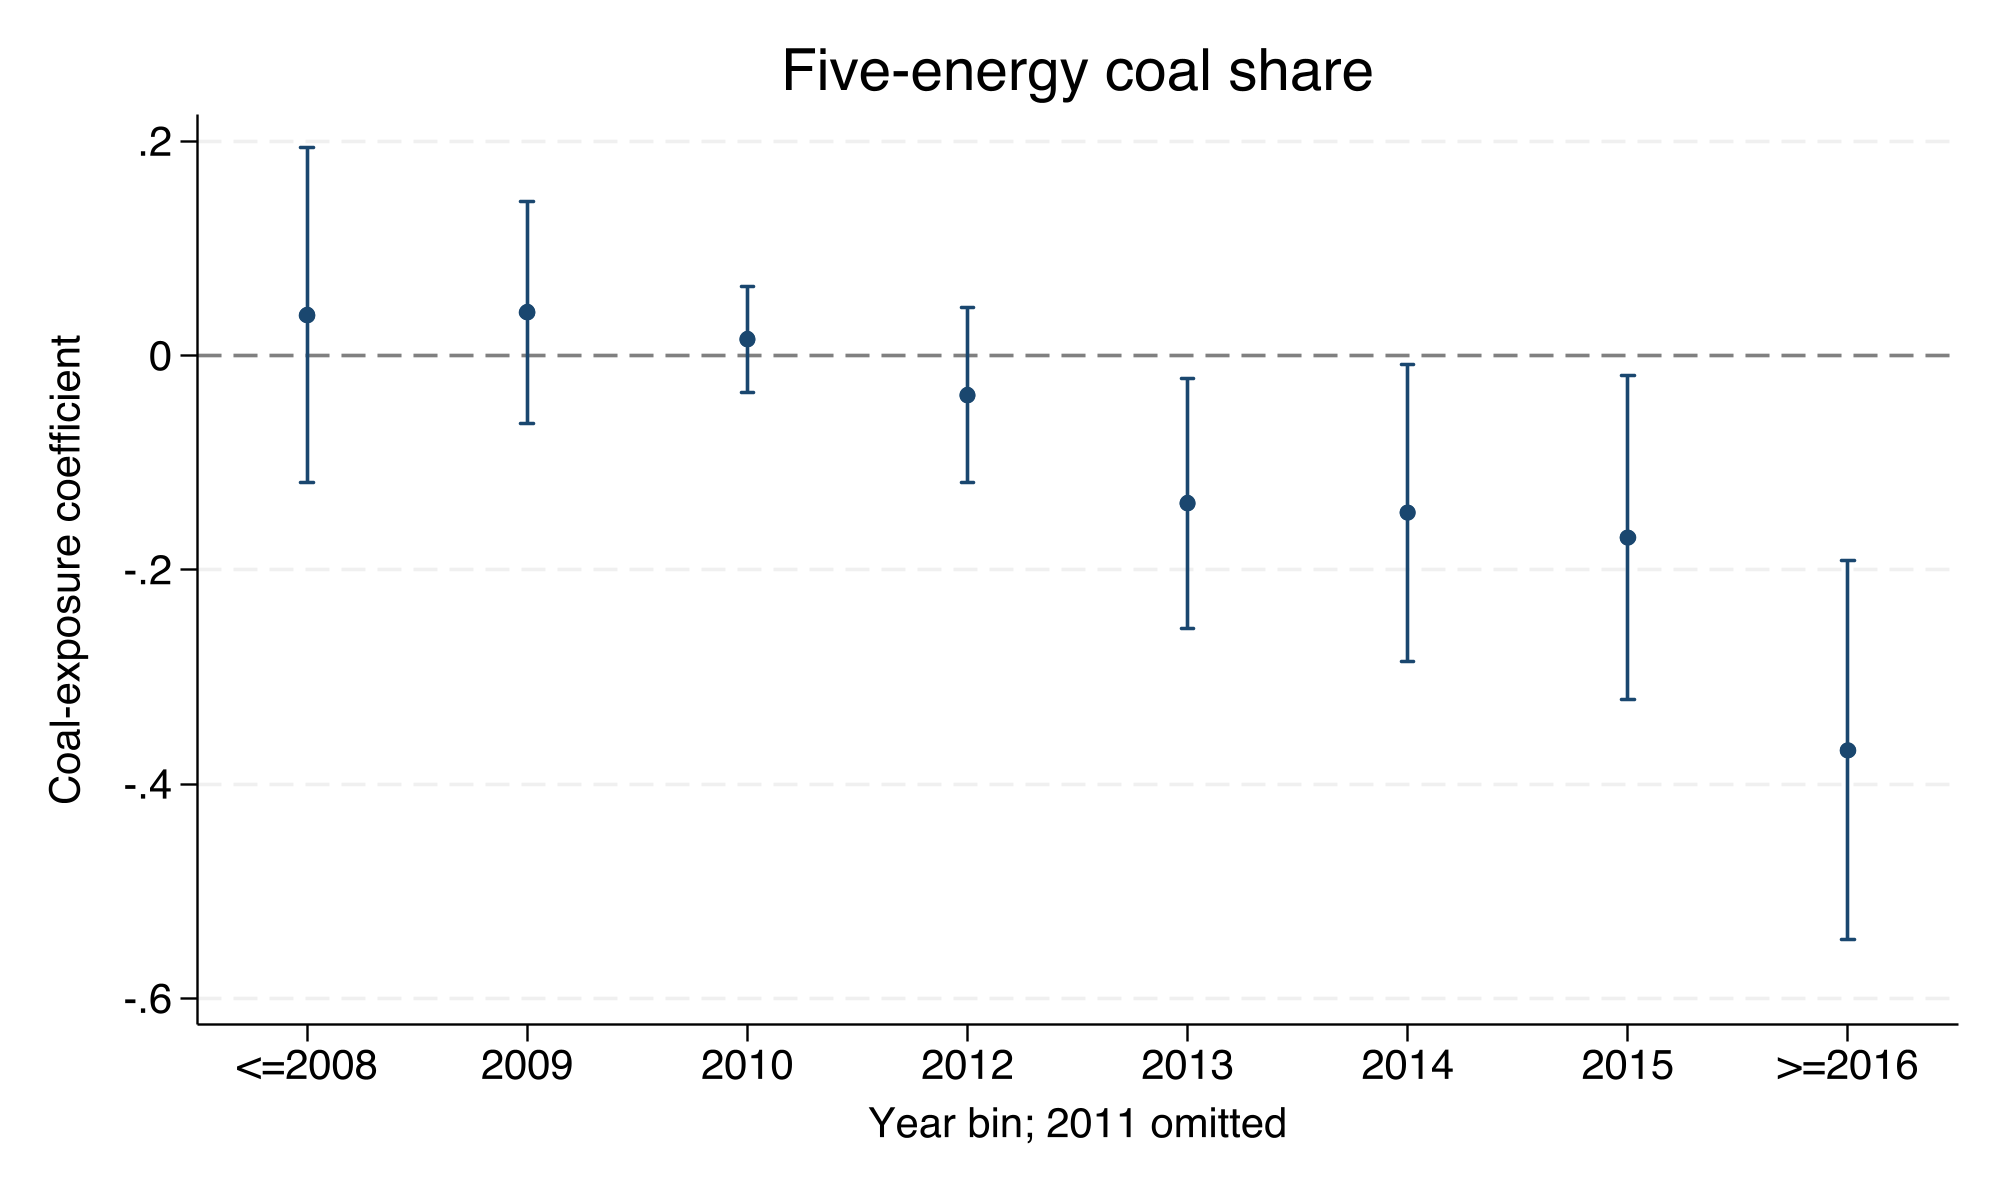
\includegraphics[width=\linewidth]{../result/figures/0718_manuscript_revision/EventStudy_coalshare5.png}
\caption{五类能源煤炭占比}
\end{subfigure}
\begin{subfigure}{0.49\textwidth}
\centering
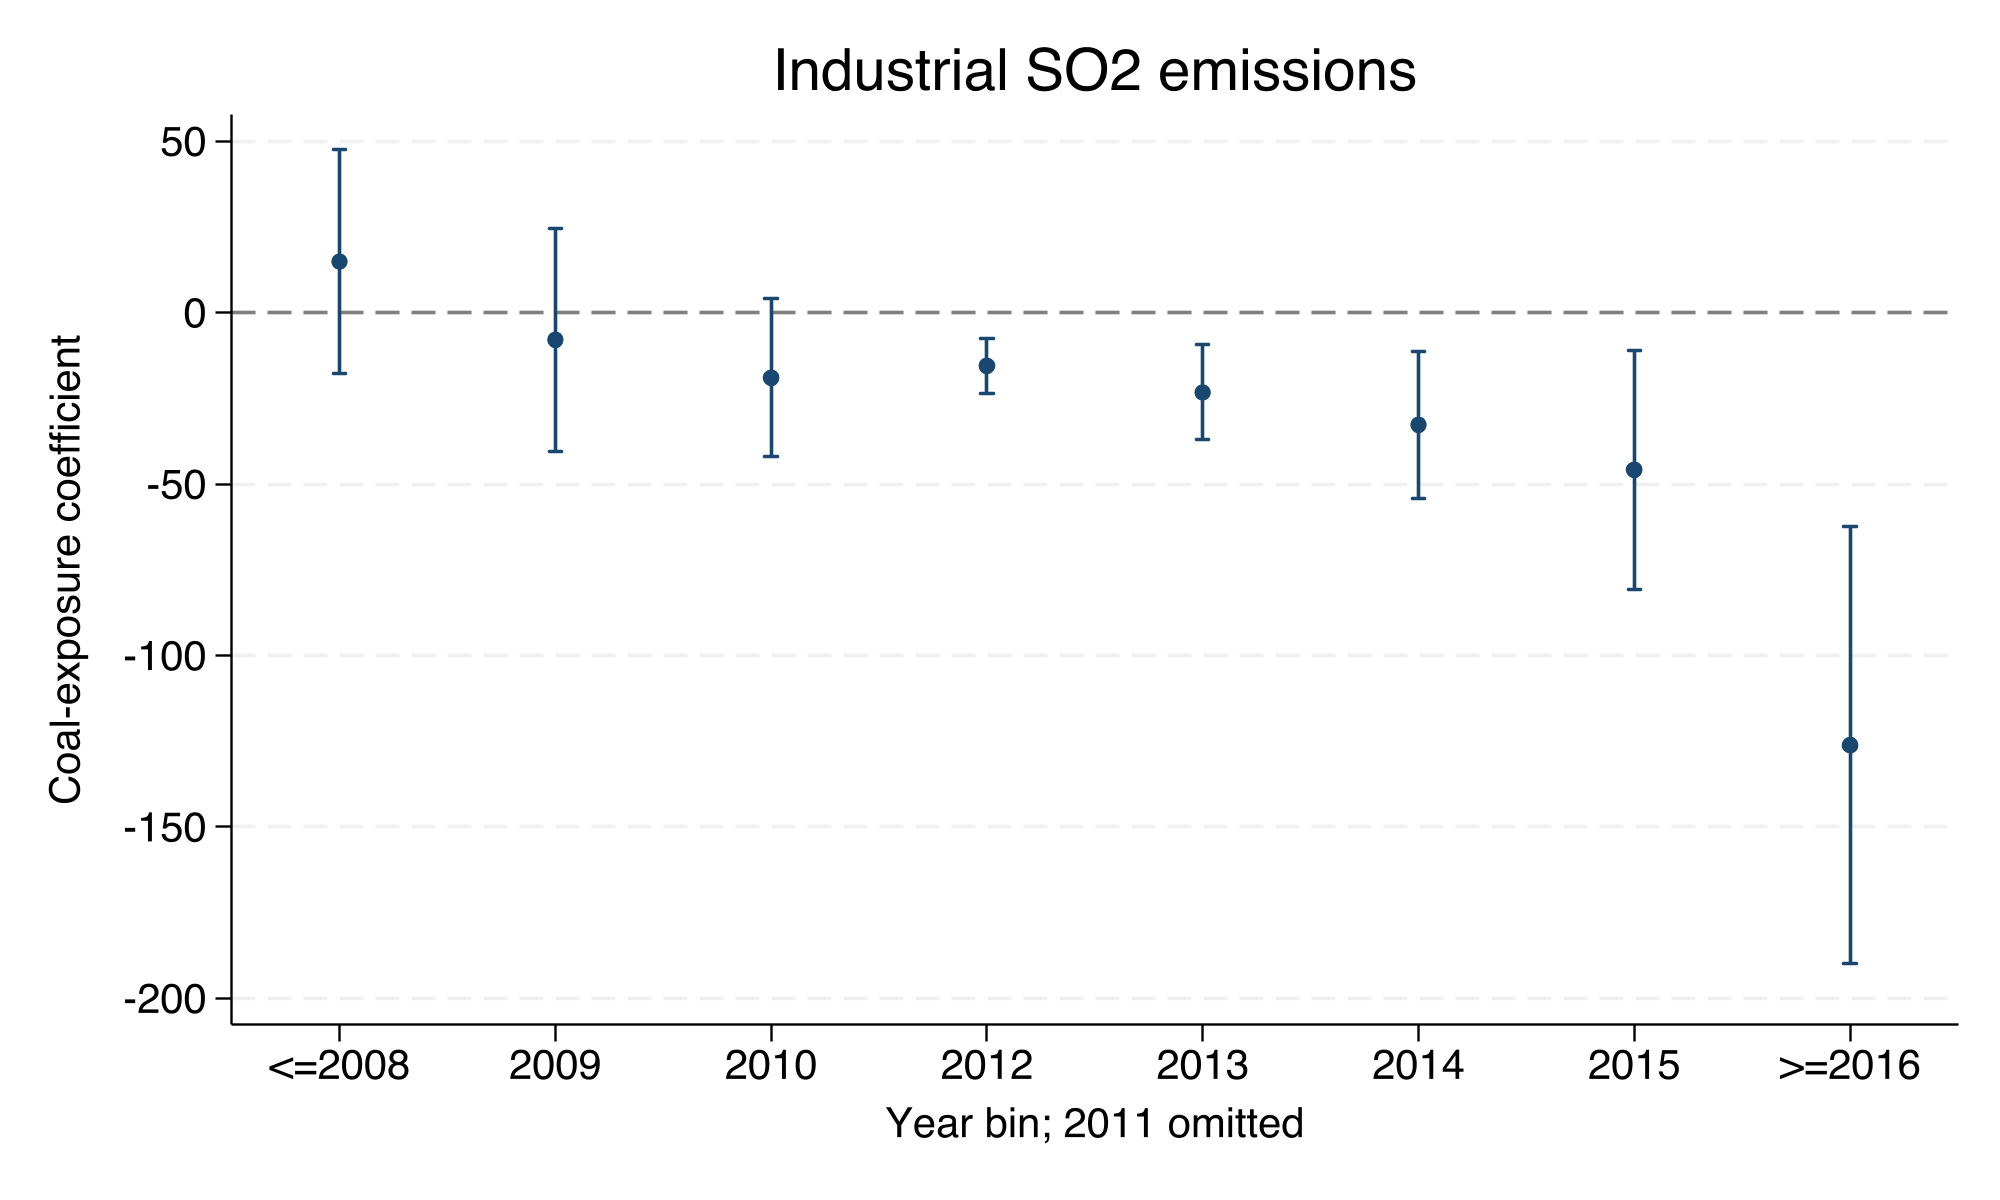
\includegraphics[width=\linewidth]{../result/figures/0718_manuscript_revision/EventStudy_industrial_so2.png}
\caption{工业SO$_2$}
\end{subfigure}
\caption{连续煤炭暴露度事件研究}
\label{fig:event}
\note{2011年为基准期；最左一档为2008年及以前，最右一档为2016年及以后。误差线为95\%置信区间。}
\end{figure}

\section{补充结果与数据覆盖}

\begin{table}[H]
\centering
\caption{绿色信贷代理的金融端诊断}
\begin{tabular}{lrrr}
\toprule
模型/结果 & 系数 & 标准误 & $p$值 \\
\midrule
政策后煤炭暴露 $\rightarrow$ 绿色信贷代理 & 0.0809 & 0.0948 & 0.401 \\
剔除2017年 & 0.0810 & 0.0913 & 0.382 \\
绿色信贷代理 $\rightarrow$ 五类能源强度 & -0.0071 & 0.0124 & 0.568 \\
绿色信贷代理 $\rightarrow$ 煤炭终端强度 & -0.0129 & 0.0116 & 0.277 \\
绿色信贷代理 $\rightarrow$ 工业SO$_2$ & 0.0379 & 3.6752 & 0.992 \\
绿色信贷代理 $\rightarrow$ 煤炭占比 & -0.0145 & 0.0112 & 0.207 \\
绿色信贷代理 $\rightarrow$ CO$_2$排放对数 & -0.0246 & 0.0121 & 0.052 \\
绿色信贷代理 $\rightarrow$ 风光发电占比 & 0.0057 & 0.0047 & 0.234 \\
\bottomrule
\end{tabular}
\note{所有模型包含省份和年份固定效应及基准控制变量。该表为相关性诊断。}
\end{table}

\begin{table}[H]
\centering
\caption{地方基础设施变量的时间覆盖}
\begin{tabular}{lrrr}
\toprule
变量 & 起始年 & 截止年 & 省年观测 \\
\midrule
省际输出电量（1--11月累计） & 2015 & 2023 & 277 \\
风电利用小时 & 2018 & 2023 & 186 \\
太阳能利用小时（1--11月累计） & 2018 & 2023 & 186 \\
风电利用率/弃风率 & 2020 & 2023 & 124 \\
光伏利用率/弃光率 & 2020 & 2023 & 124 \\
\bottomrule
\end{tabular}
\note{覆盖期均晚于2012年，不适合作为全国主模型中的先验条件。}
\end{table}

\printbibliography[title={参考文献}]

\end{document}
